
To build up the relationship among the probability theory, statistical thermodynamics and ML/AI model training, we need to introduce some of the basic concepts of the information theory, which provides us with the mathematical language to measure the information content, its associated uncertainties and how to reliably communicate information under the presence of noises, as one of the primary goal for developing ML techniques is to reduce and filter out the uncertainties in the information through model training. 

In the language of information theory, the \emph{information entropy} (or the \emph{Shannon entropy)} provides the mathematical measurement of the information uncertainty associated with the probability distribution of the information. For a continuous distribution, the information entropy is defined as
\begin{equation}
    \label{eq:information_entropy}
    S=-\int p(\bm{x})\log p(\bm{x})\mbox{d}\bm{x}=\mathbb{E}_{\bm{x}\sim p(\bm{x})}\left[-\log p(\bm{x})\right].
\end{equation}


With the idea of information content, training a ML/AI model is a \textit{process that maximises the information content overlap between the model and the training data}, and this information overlap is measured in terms of the dissimilarity between two probability distributions $p(x)$ and $q(x)$, that can be quantified using the \textit{Kullback–Leibler (KL) divergence}:
\begin{equation}
    \label{eq:KL_divergence}
    \mathcal{D}_{KL}(p||q)=\sum_{i=1}^{N}p_i\log\frac{p_i}{q_i}\qquad\mbox{or}\qquad \mathcal{D}_{KL}(p||q)=\int p(x)\log\frac{p(x)}{q(x)}\mbox{d}x.
\end{equation}
If one of the distribution is modelled by a ML/AI model with parameter(s) $\boldsymbol{\theta}$, then the model training is essentially a process to minimise the KL-divergence between the target and model distributions with respect to $\boldsymbol{\theta}$:
\begin{equation}
    \label{eq:training_KL_minimise}
    \hat{\boldsymbol{\theta}}_{\mathrm{opt}} = \argmin_{\boldsymbol{\theta}}\mathcal{D}_{KL} \left(p_{\mathrm{target}}|q_{\boldsymbol{\theta}}\right),
\end{equation}
and to simplify the training, many model tend to choose simple distributions $q_{\boldsymbol{\theta}}$ such as those listed in \cref{tab:discrete_prob_distributions} and \cref{tab:continuous_prob_distributions} to derive analytical expressions for $\mathcal{D}_{KL}$ that are easy to compute. We shall provide more concrete examples of applying this in the following sections.  A simple example is shown here in \cref{fig:KL_div_normal} which shows how KL-divergence changes between parameterised one-dimensional normal distribution $\mathcal{N}(\mu,\sigma^2)$ with respect to the standard normal distribution $\mathcal{N}(0,1)$ as a function of the mean and variance. 




\begin{figure}[tbh]
\centering
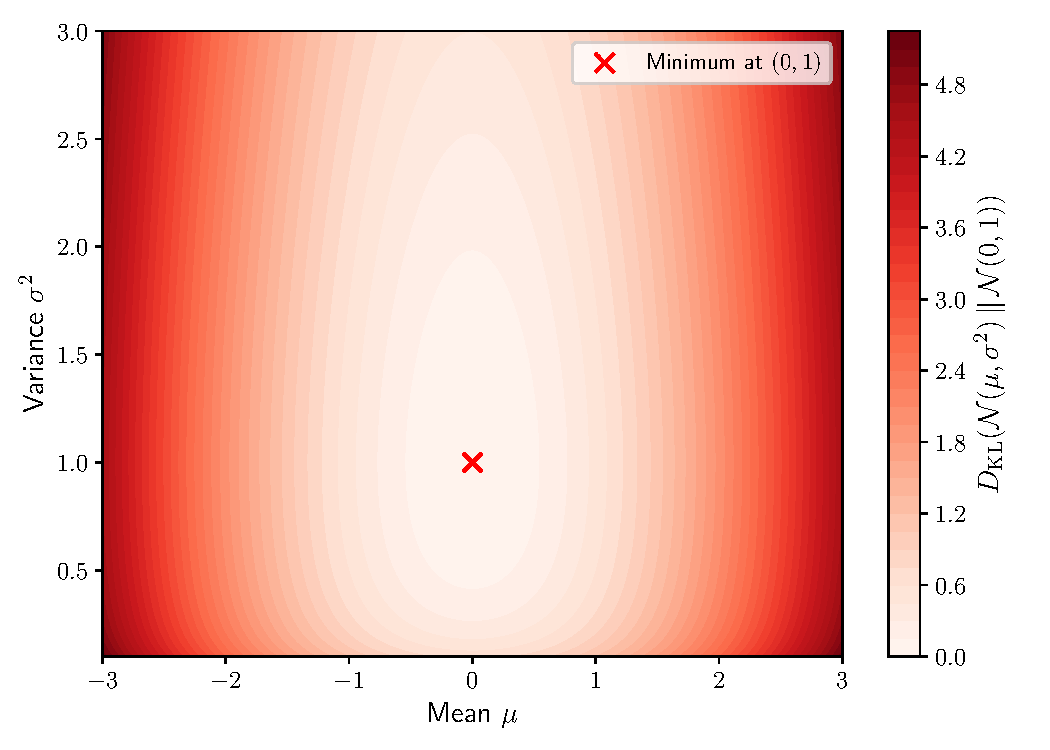
\includegraphics[width=0.5\linewidth]{KL_div_normal.pdf}
\caption{Landscape of the KL divergence between a parameterised one-dimensional normal distribution $\mathcal{N}(\mu,\sigma^2)$ and a standard normal distribution $\mathcal{N}(0,1)$ as a function of the mean ($\mu$) and variance ($\sigma^2$).} 
\label{fig:KL_div_normal} 
\end{figure}

Alternatively, in many ML/AI literatures, instead of minimising the KL-divergences between two probability distributions, the problem is often reformulated into an opposite problem of \emph{maximising the log-likelihood} between two distributions. By expanding
\begin{equation}
    \label{eq:DKL_expand}
    \mathcal{D}_{KL}(p||q)=\sum_i p_i\log p_i-\sum_i p_i\log q_{i,\boldsymbol{\theta}},
\end{equation}
and realising that the first term on the right hand side is essentially a constant, the optimal model parameter $\boldsymbol{\theta}$ can therefore be obtained equivalently by maximising the log-likelihood function $\sum_i p_i\log q_{i,\boldsymbol{\theta}}$.

%To provide more physical context behind the definitions of KL-divergence [\cref{eq:KL_divergence}], we re-examine the probabilistic interpretation behind the anharmonicity score defined in \cref{eq:anharmonic_score}. 
